% move all configuration stuff into includes file so we can focus on the content
\documentclass[aspectratio=169,hyperref={pdfpagelabels=false,colorlinks=true,linkcolor=white,urlcolor=blue},t]{beamer}

%%%%%%%%%%%%%%%%%%%%%%%%%%%%%%%%%%%%%%%%%%%%%%%%%%%%%%%%%%%%%%%%%%%%%%%%%%%%%%%%%%
%%%%%%%%%%%%%%%%%%%%%%%%%%%%%%%%%%%%%%%%%%%%%%%%%%%%%%%%%%%%%%%%%%%%%%%%%%%%%%%%%%
% packages
\usepackage{pict2e}
\usepackage{epic}
\usepackage{amsmath,amsfonts,amssymb}
\usepackage{units}
\usepackage{fancybox}
\usepackage[absolute,overlay]{textpos} 
\usepackage{media9} % avi2flv: "C:\Program Files\ffmpeg\bin\ffmpeg.exe" -i TuneFreqFilterbank.avi -b 600k -s 441x324 -r 15 -acodec copy TuneFreqFilterbank.flv
\usepackage{animate}
\usepackage{gensymb}
\usepackage{multirow}
\usepackage{silence}
\usepackage[backend=bibtex,style=ieee]{biblatex}
\AtEveryCitekey{\iffootnote{\tiny}{}}
\addbibresource{references}

%%%%%%%%%%%%%%%%%%%%%%%%%%%%%%%%%%%%%%%%%%%%%%%%%%%%%%%%%%%%%%%%%%%%%%%%%%%%%%%%%%
%%%%%%%%%%%%%%%%%%%%%%%%%%%%%%%%%%%%%%%%%%%%%%%%%%%%%%%%%%%%%%%%%%%%%%%%%%%%%%%%%%
% relative paths
\graphicspath{{graph/}}


%%%%%%%%%%%%%%%%%%%%%%%%%%%%%%%%%%%%%%%%%%%%%%%%%%%%%%%%%%%%%%%%%%%%%%%%%%%%%%%%%%
%%%%%%%%%%%%%%%%%%%%%%%%%%%%%%%%%%%%%%%%%%%%%%%%%%%%%%%%%%%%%%%%%%%%%%%%%%%%%%%%%%
% units
\setlength{\unitlength}{1mm}

%%%%%%%%%%%%%%%%%%%%%%%%%%%%%%%%%%%%%%%%%%%%%%%%%%%%%%%%%%%%%%%%%%%%%%%%%%%%%%%%%%
%%%%%%%%%%%%%%%%%%%%%%%%%%%%%%%%%%%%%%%%%%%%%%%%%%%%%%%%%%%%%%%%%%%%%%%%%%%%%%%%%%
% theme & layout
\usetheme{Frankfurt}
\beamertemplatenavigationsymbolsempty
%\setbeamertemplate{frametitle}[smoothbars theme]
\setbeamertemplate{frametitle}
{
    \begin{beamercolorbox}[ht=1.8em,wd=\paperwidth]{frametitle}
        \vspace{-.1em}%
        \hspace{.2em}{\strut\insertframetitle\strut}
        
        \hspace{.2em}\small\strut\insertframesubtitle\strut
        %\hfill
        %
\includegraphics[height=.8cm,keepaspectratio]{CenterMusicTechnology-solid-2lines-white-CoAtag}
        
    \end{beamercolorbox}
    \begin{textblock*}{100mm}(11.6cm,.7cm)
        \includegraphics[height=.8cm,keepaspectratio]{logo_GTCMT_black}
    \end{textblock*}
}

% set this to ensure bulletpoints without subsections
\usepackage{remreset}
\makeatletter
\@removefromreset{subsection}{section}
\makeatother
\setcounter{subsection}{1}

%---------------------------------------------------------------------------------
% appearance
\setbeamercolor{structure}{fg=gtgold}
\setbeamercovered{transparent} %invisible
\setbeamercolor{bibliography entry author}{fg=black}
\setbeamercolor*{bibliography entry title}{fg=black}
\setbeamercolor*{bibliography entry note}{fg=black}

%\usepackage{pgfpages}
%\setbeameroption{show notes}
%\setbeameroption{show notes on second screen=right}
%---------------------------------------------------------------------------------
% fontsize
\let\Tiny=\tiny

%%%%%%%%%%%%%%%%%%%%%%%%%%%%%%%%%%%%%%%%%%%%%%%%%%%%%%%%%%%%%%%%%%%%%%%%%%%%%%%%%%
%%%%%%%%%%%%%%%%%%%%%%%%%%%%%%%%%%%%%%%%%%%%%%%%%%%%%%%%%%%%%%%%%%%%%%%%%%%%%%%%%%
% warnings
\pdfsuppresswarningpagegroup=1
\WarningFilter{biblatex}{Patching footnotes failed}
\WarningFilter{latexfont}{Font shape}
\WarningFilter{latexfont}{Some font shapes}
\WarningFilter{gensymb}{Not defining}


%%%%%%%%%%%%%%%%%%%%%%%%%%%%%%%%%%%%%%%%%%%%%%%%%%%%%%%%%%%%%%%%%%%%%%%%%%%%%%%%%%
%%%%%%%%%%%%%%%%%%%%%%%%%%%%%%%%%%%%%%%%%%%%%%%%%%%%%%%%%%%%%%%%%%%%%%%%%%%%%%%%%%
% title information
\title[]{Introduction to Audio Content Analysis}   
\author[alexander lerch]{alexander lerch} 
%\institute{~}
%\date[Alexander Lerch]{}
\titlegraphic{\vspace{-16mm}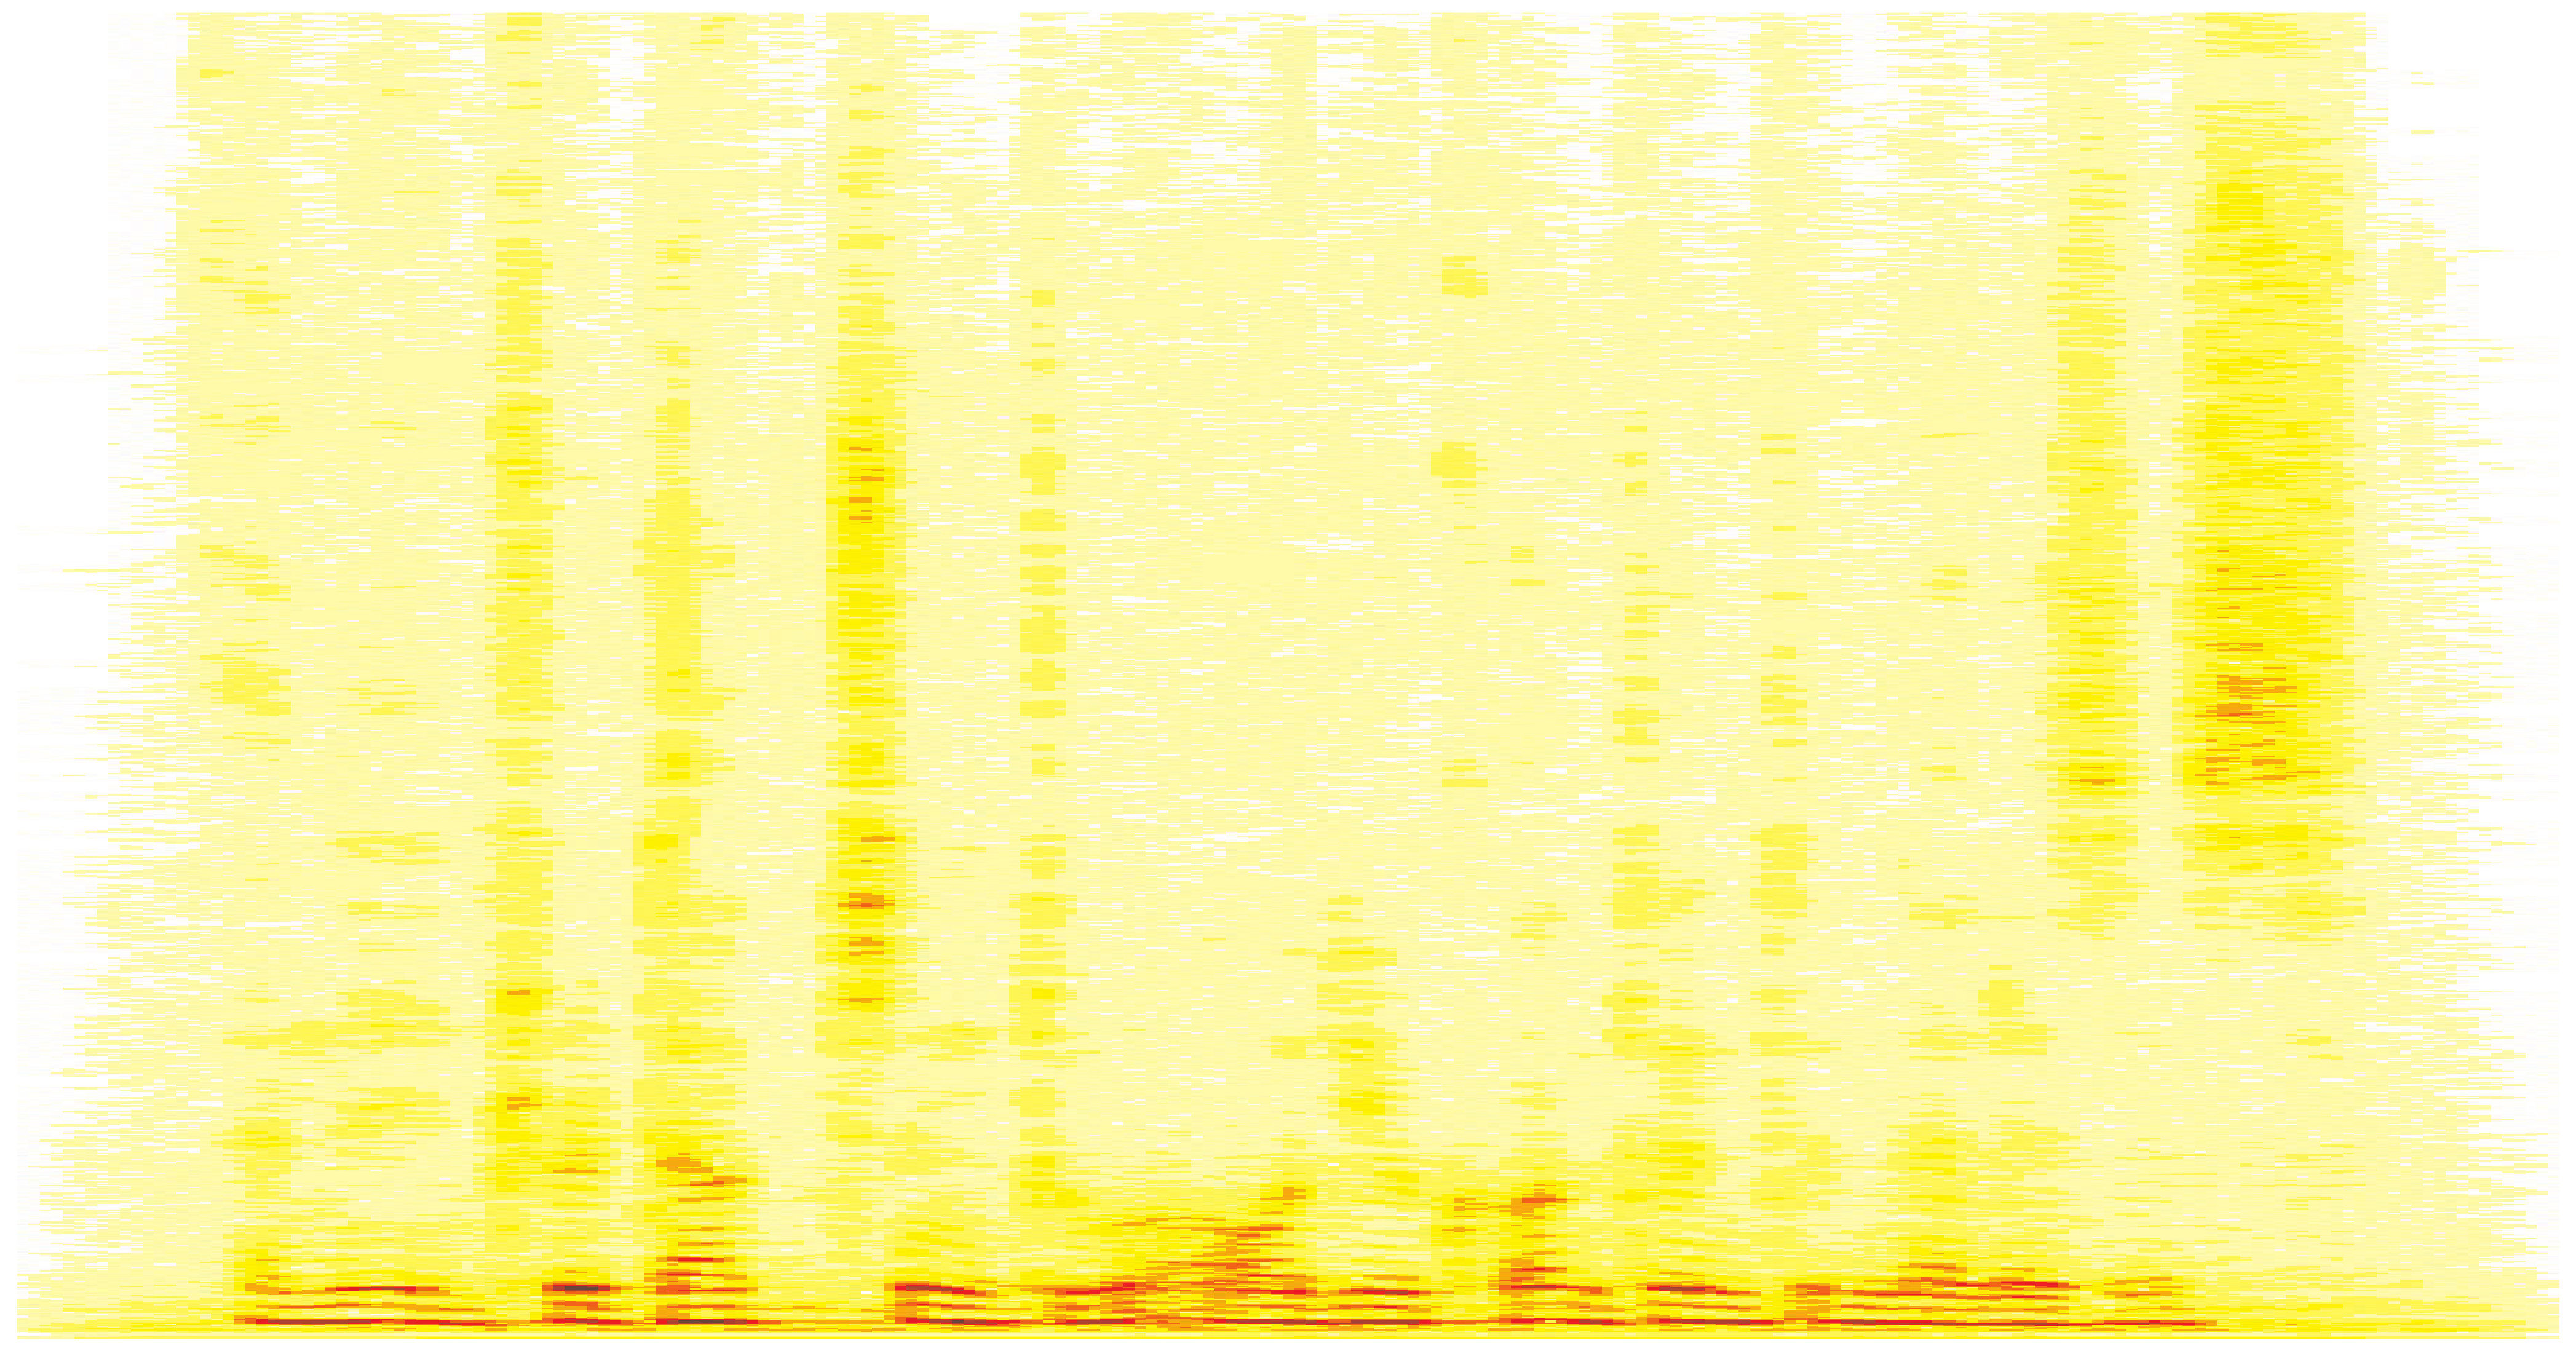
\includegraphics[width=\textwidth,height=3cm]{title}}

%%%%%%%%%%%%%%%%%%%%%%%%%%%%%%%%%%%%%%%%%%%%%%%%%%%%%%%%%%%%%%%%%%%%%%%%%%%%%%%%%%
%%%%%%%%%%%%%%%%%%%%%%%%%%%%%%%%%%%%%%%%%%%%%%%%%%%%%%%%%%%%%%%%%%%%%%%%%%%%%%%%%%
% colors
\definecolor{gtgold}{HTML}{E0AA0F} %{rgb}{0.88,0.66,1,0.06} [234, 170, 0]/256

%%%%%%%%%%%%%%%%%%%%%%%%%%%%%%%%%%%%%%%%%%%%%%%%%%%%%%%%%%%%%%%%%%%%%%%%%%%%%%%%%%
%%%%%%%%%%%%%%%%%%%%%%%%%%%%%%%%%%%%%%%%%%%%%%%%%%%%%%%%%%%%%%%%%%%%%%%%%%%%%%%%%%
% math
\DeclareMathOperator*{\argmax}{argmax}
\DeclareMathOperator*{\argmin}{argmin}
\DeclareMathOperator*{\atan}{atan}
\DeclareMathOperator*{\arcsinh}{arcsinh}
\DeclareMathOperator*{\sign}{sign}
\DeclareMathOperator*{\tcdf}{tcdf}
\DeclareMathOperator*{\si}{sinc}
\DeclareMathOperator*{\princarg}{princarg}
\DeclareMathOperator*{\arccosh}{arccosh}
\DeclareMathOperator*{\hwr}{HWR}
\DeclareMathOperator*{\flip}{flip}
\DeclareMathOperator*{\sinc}{sinc}
\DeclareMathOperator*{\floor}{floor}
\newcommand{\e}{{e}}
\newcommand{\jom}{\mathrm{j}\omega}
\newcommand{\jOm}{\mathrm{j}\Omega}
\newcommand   {\mat}[1]    		{\boldsymbol{\uppercase{#1}}}		%bold
\renewcommand {\vec}[1]    		{\boldsymbol{\lowercase{#1}}}		%bold

%%%%%%%%%%%%%%%%%%%%%%%%%%%%%%%%%%%%%%%%%%%%%%%%%%%%%%%%%%%%%%%%%%%%%%%%%%%%%%%%%%
%%%%%%%%%%%%%%%%%%%%%%%%%%%%%%%%%%%%%%%%%%%%%%%%%%%%%%%%%%%%%%%%%%%%%%%%%%%%%%%%%%
% media9
\newcommand{\includeaudio}[1]{{\includemedia[
                        addresource=audio/#1.mp3,
                        width=5mm,
                        height=5mm,
                        activate=onclick,
                        flashvars={
                            source=audio/#1.mp3  
                            &autoPlay=true
                        }]
                        {
\includegraphics[width=5mm, height=5mm]{SpeakerIcon}}
                        {APlayer.swf}}}
\newcommand{\audioautoplay}[1]{{\begin{center}\includemedia[
                            addresource=audio/#1.mp3,
                            width=.1\linewidth,
                            height=.01\linewidth,
                            activate=pageopen,
                            flashvars={
                                source=audio/#1.mp3  
                                &autoPlay=true
                            }]
                            {}
                            {APlayer.swf}\end{center}}}

\newcommand{\includevideo}[1]{{\begin{center}\includemedia[
                        addresource=video/#1.mp4,
                        width=0.8\linewidth,
                        height=0.4\linewidth,
                        activate=onclick,
                        flashvars={
                            source=video/#1.mp4  
                            &autoPlay=true
                        }]
                        {}
                        {VPlayer.swf}\end{center}}}
\newcommand{\videowithmatlab}[1]{{\begin{center}\includemedia[
                        addresource=video/animate#1.mp4,
                        width=0.8\linewidth,
                        height=0.4\linewidth,
                        activate=onclick,
                        flashvars={
                            source=video/animate#1.mp4  
                            &autoPlay=true
                        }]
                        {}
                        {VPlayer.swf}\end{center}\addreference{matlab source: matlab/animate#1.m}}}
                        

%%%%%%%%%%%%%%%%%%%%%%%%%%%%%%%%%%%%%%%%%%%%%%%%%%%%%%%%%%%%%%%%%%%%%%%%%%%%%%%%%%
%%%%%%%%%%%%%%%%%%%%%%%%%%%%%%%%%%%%%%%%%%%%%%%%%%%%%%%%%%%%%%%%%%%%%%%%%%%%%%%%%%
% other commands
\newcommand{\question}[1]{%\vspace{-4mm}
                          \setbeamercovered{invisible}
                          \begin{columns}[T]
                            \column{.8\textwidth}
                                \textbf{#1}
                            \column{.2\textwidth}
                                \vspace{-8mm}
                                \begin{flushright}
                                     
\includegraphics[scale=.5]{question_mark}
                                \end{flushright}
                                \vspace{6mm}
                          \end{columns}\pause\vspace{-12mm}}

\newcommand{\toremember}[1]{%\vspace{-4mm}
                          \begin{columns}[T]
                            \column{.8\textwidth}
                                \textbf{#1}
                            \column{.2\textwidth}
                                \vspace{-4mm}
                                \begin{flushright}
                                     
\includegraphics[scale=.5]{exclamation_mark}
                                \end{flushright}
                                \vspace{6mm}
                          \end{columns}\vspace{-6mm}}

\newcommand{\matlabexercise}[1]{%\vspace{-4mm}
                          \setbeamercovered{invisible}
                          \begin{columns}[T]
                            \column{.8\textwidth}
                                \textbf{matlab exercise}: #1
                            \column{.2\textwidth}
                                \begin{flushright}
                                     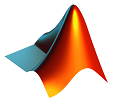
\includegraphics[scale=.5]{logo_matlab}
                                \end{flushright}
                                %\vspace{6mm}
                          \end{columns}}

\newcommand{\addreference}[1]{  
                  
                    \begin{textblock*}{\baselineskip }(1.12\textwidth,.3\textheight) %(1.15\textwidth,.4\textheight)
                        \rotatebox{90}{\tiny {#1}}
                    \end{textblock*}}
                    
\newcommand{\figwithmatlab}[1]{
                    \begin{figure}
                        \centering
                        \includegraphics{#1}
                        %\label{fig:#1}
                    \end{figure}
                    
                    \addreference{matlab source: \href{https://github.com/alexanderlerch/ACA-Slides/blob/master/matlab/display#1.m}{matlab/display#1.m}}}
\newcommand{\figwithref}[2]{
                    \begin{figure}
                        \centering
                        \includegraphics{#1}
                        \label{fig:#1}
                    \end{figure}
                    
                    \addreference{#2}}  
                                    
\newcommand{\inserticon}[1]{

                    \begin{textblock*}{100mm}(14.5cm,7.5cm)
                        \includegraphics[height=.8cm,keepaspectratio]{#1}
                    \end{textblock*}}            

%%%%%%%%%%%%%%%%%%%%%%%%%%%%%%%%%%%%%%%%%%%%%%%%%%%%%%%%%%%%%%%%%%%%%%%%%%%%%%%%%%
%%%%%%%%%%%%%%%%%%%%%%%%%%%%%%%%%%%%%%%%%%%%%%%%%%%%%%%%%%%%%%%%%%%%%%%%%%%%%%%%%%
% counters
\newcounter{i}
\newcounter{j}
\newcounter{iXOffset}
\newcounter{iYOffset}
\newcounter{iXBlockSize}
\newcounter{iYBlockSize}
\newcounter{iYBlockSizeDiv2}
\newcounter{iDistance}



\subtitle{Module 7.1: Audio-to-Audio \& Audio-to-Score Alignment}

%%%%%%%%%%%%%%%%%%%%%%%%%%%%%%%%%%%%%%%%%%%%%%%%%%%%%%%%%%%%%%%%%%%%%%%%%%%%
\begin{document}
    % generate title page
	

\begin{frame}
    \titlepage
    %\vspace{-5mm}
    \begin{flushright}
        \href{http://www.gtcmt.gatech.edu}{\includegraphics[height=.8cm,keepaspectratio]{logo_GTCMT_black}}
    \end{flushright}
\end{frame}


    \section[overview]{lecture overview}
        \begin{frame}{introduction}{overview}
            \begin{block}{corresponding textbook section}
                    \href{http://ieeexplore.ieee.org/xpl/articleDetails.jsp?arnumber=6331124}{Chapter 7: Alignment} (pp.~146--150)
            \end{block}

            \begin{itemize}
                \item   \textbf{lecture content}
                    \begin{itemize}
                        \item   Dynamic Time Warping (DTW):
                        \item[] synchronization of two sequences with similar content
                    \end{itemize}
                \bigskip
                \item<2->   \textbf{learning objectives}
                    \begin{itemize}
                        \item   explain the standard DTW algorithm
                        \item   discuss disadvantages of and modifications to the standard DTW algorithm
                        \item   implement DTW
                    \end{itemize}
            \end{itemize}
            \inserticon{directions}
        \end{frame}

    \section[A2A]{Audio to audio alignment}
        \begin{frame}{audio-to-audio alignment}{introduction}
            \begin{itemize}
                \item	\textbf{objective}
                    \begin{itemize}
                        \item	align two sequences of audio
                    \end{itemize}
                \bigskip
                \item<2->	\textbf{use cases}
                    \begin{itemize}
                        \item	\textit{quick browsing} for certain parts in recordings
                        \item	\textit{timing adjustment} (backing vocals, loops, \ldots)
                        \item	\textit{automated dubbing}
                        \item	\textit{musicological analysis} (timing of several performances)
                    \end{itemize}
                \bigskip
                \item<3->	\textbf{processing steps}
                    \begin{itemize}
                        \item	extract suitable features
                        \item	compute distance matrix
                        \item	compute alignment path
                    \end{itemize}
            \end{itemize}
        \end{frame}

        \begin{frame}{audio-to-audio alignment}{alignment path computation}
            \vspace{-2mm}
            $\rightarrow$ prerequisite: Module 7.0---Dynamic Time Warping
            \vspace{-3mm}
            \figwithmatlab{Dtw}
        \end{frame}

        \begin{frame}{audio-to-audio alignment}{features}
            \vspace{-2mm}
            \only<1-2>{
                \begin{itemize}
                    \item	\textbf{use case examples}
                        \begin{itemize}
                            \item	\textbf{quick browsing} --- find the same part across files\\
                                $\Rightarrow$ use \textit{pitch based} features
                            \item	\textbf{timing adjustment} --- backing vocals to lead vocals\\
                                $\Rightarrow$ use \textit{intensity based} features
                            \item	\textbf{automated dubbing} --- same speaker several recordings\\
                                $\Rightarrow$ use \textit{intensity based} and \textit{timbre based} features
                        \end{itemize}
                    \smallskip
                    \item<2-> \textbf{feature categories}
                        \begin{itemize}
                            \item	\textbf{intensity}: energy, onset probability, \ldots
                            \item	\textbf{tonal}: pitch chroma, \ldots
                            \item	\textbf{timbral}: MFCCs, spectral shape, \ldots
                        \end{itemize}
                    \item<2->[] plot from \footfullcite{kirchhoff_evaluation_2011}
                \end{itemize}
            }
            \only<3>{
                \begin{figure}
                    \centerline{\includegraphics[scale=.5]{graph/ATAA_features}}
                \end{figure}
            }
        \end{frame}
        
        \begin{frame}{audio-to-audio alignment}{compute distance matrix --- distance measures}
            \begin{itemize}
                \item	typical distance measures
                    \only<1-4>{
                    \begin{itemize}
                        \item<1-4>	\emph{{Euclidean distance}}:
                                $d_\mathrm{E}(s) = \sqrt{\sum\limits_{j = 0}^{11}{\big(\nu_\mathrm{e}(j)-\nu_\mathrm{t,s}(j)\big)^2}} $
                        \item<2-4>	\emph{{Manhattan distance}}:
                                $d_\mathrm{M}(s) = \sum\limits_{j = 0}^{11}{\big|\nu_\mathrm{e}(j)-\nu_\mathrm{t,s}(j)\big|} $
                        \item<3-4>	\emph{{Cosine distance}}:
                                $d_\mathrm{C}(s) = 1-\left( \frac{\sum\limits_{j = 0}^{11}{\nu_\mathrm{e}(j)\cdot\nu_\mathrm{t,s}(j)}}{\sqrt{\sum\limits_{j = 0}^{11}{\nu_\mathrm{e}(j)^2}}\sqrt{\cdot \sum\limits_{j = 0}^{11}{\nu_\mathrm{t,s}(j)^2}}}\right) $
                        \item<4-4>	\emph{{Kullback-Leibler divergence}}:
                                $d_\mathrm{KL}(s) = \sum\limits_{j = 0}^{11}{\nu_\mathrm{e}(j)\cdot\log\left(\frac{\nu_\mathrm{e}(j)}{\nu_\mathrm{t,s}(j)}\right)}$
                    \end{itemize}
                    }
                \smallskip
                \item<5->	data-driven approach: train classifier with 2-class problem \footfullcite{kirchhoff_evaluation_2011}
                    \only<5>{
                        \begin{figure}
                            \centerline{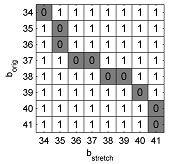
\includegraphics[scale=.5]{graph/ATAA_feature_training}}
                        \end{figure}
                    }
                    \only<6>{
                        \begin{figure}
                            \centerline{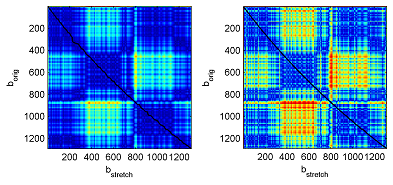
\includegraphics[scale=.5]{graph/ATAA_simmatrix_compare}}
                        \end{figure}
                    }
            \end{itemize}
        \end{frame}
        
        \begin{frame}{audio-to-audio alignment}{typical results}
            \vspace{-5mm}
            \begin{columns}
            \column{.7\linewidth}
                \vspace{-3mm}\begin{figure}
                    \centerline{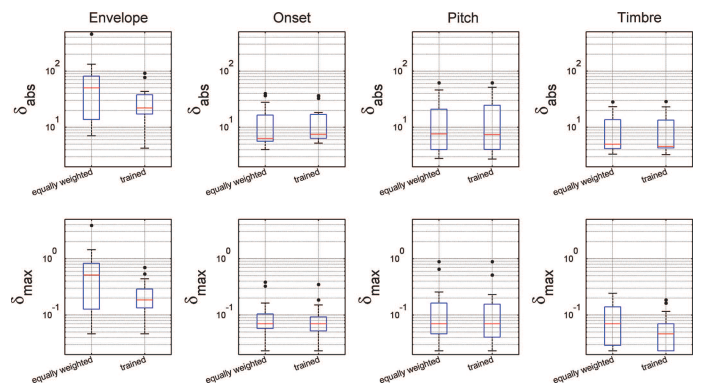
\includegraphics[width= \columnwidth]{graph/ATAA_results}}
                \end{figure}
            \column{.3\linewidth}
                \begin{table}
                    \begin{tabular}{p{.55\columnwidth}l}
                        \textbf{originals}\linebreak
                        \begin{scriptsize}
                            left:~instrumental\hfill \linebreak
                            right:~a capella
                        \end{scriptsize} & \textbf{synced}\\
                        \includeaudio{originals_splanky} & \includeaudio{synced_splanky}
                    
                    \end{tabular}
                \end{table}
            \end{columns}
            \footfullcite{kirchhoff_evaluation_2011}
            \inserticon{audio}
        \end{frame}
        
    \section[A2S]{Audio to score alignment}
        \begin{frame}{audio-to-score alignment}{overview}
            \begin{itemize}
                \item   \textbf{objective}
                    \begin{itemize}
                        \item align an audio sequence with a score sequence
                    \end{itemize}
                \bigskip
                \item<2->   \textbf{use cases}
                    \begin{itemize}
                        \item   score viewer
                        \item   music education
                        \item   identify matching score/audio via cost function
                        \item   musicological analysis
                    \end{itemize}
                \bigskip
                \item<3->   \textbf{processing steps}
                    \begin{itemize}
                        \item   see audio-to-audio alignment
                    \end{itemize}
            \end{itemize}
        \end{frame}
        \begin{frame}{audio-to-score alignment}{challenges}
            \begin{itemize}
                \item   features from \textbf{different domains} (no timbre and proper loudness information in the score)
                    \begin{itemize}
                        \item   \textit{approach 1}: convert score into audio-like representation
                            \begin{itemize}
                                \item   MIDI-to-audio
                                \item   use model for harmonics and ADSR
                            \end{itemize}
                        \item   \textit{approach 2}: convert audio into score-like representation
                            \begin{itemize}
                                \item   audio-to-MIDI 
                                \item   pitch chroma
                                \item   event-based segmentation
                            \end{itemize}
                    \end{itemize}
                \bigskip
                \item<2->   pauses and rests
                    \begin{itemize}
                        \item   DTW algorithm has no graceful way of dealing with pauses
                    \end{itemize}
            \end{itemize}
        \end{frame}

    
    \section{summary}
        \begin{frame}{summary}{lecture content}
            \begin{itemize}
                \item   \textbf{dynamic time warping}
                    \begin{itemize}
                        \item   find globally optimal alignment path between two sequences
                    \end{itemize}
                \bigskip
                \item   \textbf{processing steps}
                    \begin{enumerate}
                        \item   compute distance matrix
                        \item   compute cost matrix
                        \item   back-track path
                    \end{enumerate}
            \end{itemize}
            \inserticon{summary}
        \end{frame}
\end{document}
